\chapter{Representation Learning and Autoencoders}

\section{Three Types of Learning}
\begin{itemize}
    \item \textbf{Supervised Learning: } 
    \begin{itemize}
        \item Use labelled data
        \item Direct feedback
        \item Predict outcome or future
    \end{itemize}
    \item \textbf{Unsupervised Learning: } 
    \begin{itemize}
        \item No data labels
        \item No feedback
        \item Find a hidden structure or group (clustering)
    \end{itemize}
    \item \textbf{Reinforcement Learning: } 
    \begin{itemize}
        \item Decision Process
        \item Rewards System
        \item Learn a series of actions
    \end{itemize}
\end{itemize}

\subsection{Labelled or Unlabelled Data?}
\subsubsection{Supervised Learning Data Requirements}
The goal of supervised learning is to learn a relation between inputs and outputs $f:\mathcal{X}\to\mathcal{Y}$ for a given number of examples $(x_i,y_i)_{i=1}^n$, The more (usable) data, the better. But labelled data can be hard to come by.

\subsubsection{Unsupervised Learning to the Rescue?}
Unsupervised learning does not need labelled data – so it is usually inexpensive to collect large training sets.

Unsupervised data automatically finds relevant patterns in input data. It reduces the complexity of a supervised learning problem as it finds only useful features from the data and discarding what is unnecessary. 

\subsubsection{Semi-supervised Learning}
Semi-supervised learning is a branch of machine learning that combines supervised and unsupervised learning by using both labelled and unlabelled data to train models for classification and regression tasks.\\

It works based on the assumption that input data encodes useful properties about the input-output relation. It then can utilise both types of data to learn the shape of the larger data distribution.

\begin{figure}[H]
    \centering
    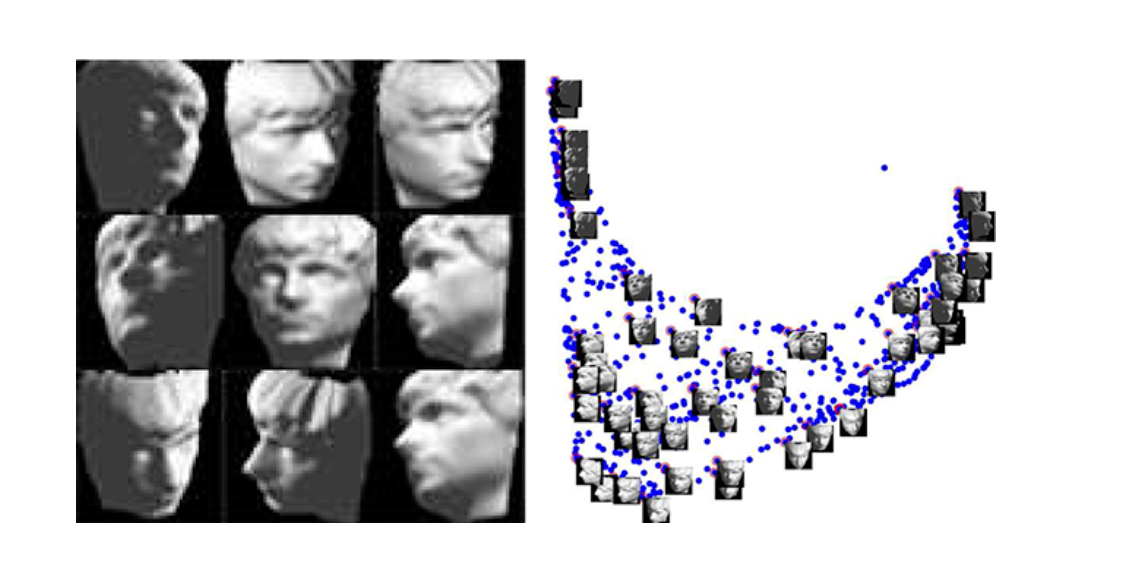
\includegraphics[width=0.5\linewidth]{img/image_face_dist.png}
    \caption{Pictures of human faces span a very low-dimensional subspace with respect to all possible images.}
\end{figure}

\subsection{Unsupervised Learning}
\begin{itemize}
    \item \textbf{Clustering: } Groups points according to common properties
    \item \textbf{Dimensionality Reduction: } Map points to a low dimensional space by keeping most of their relations unchanged
    \item \textbf{Density Estimation: } Approximate the distribution from the observed sample data, and try generate new examples of the data
    \item \textbf{Feature/Representation Learning: } Encode data within a concise but characteristic representation that can be used to solve other tasks e.g. classification, regression, etc
    \begin{figure}[H]
        \centering
        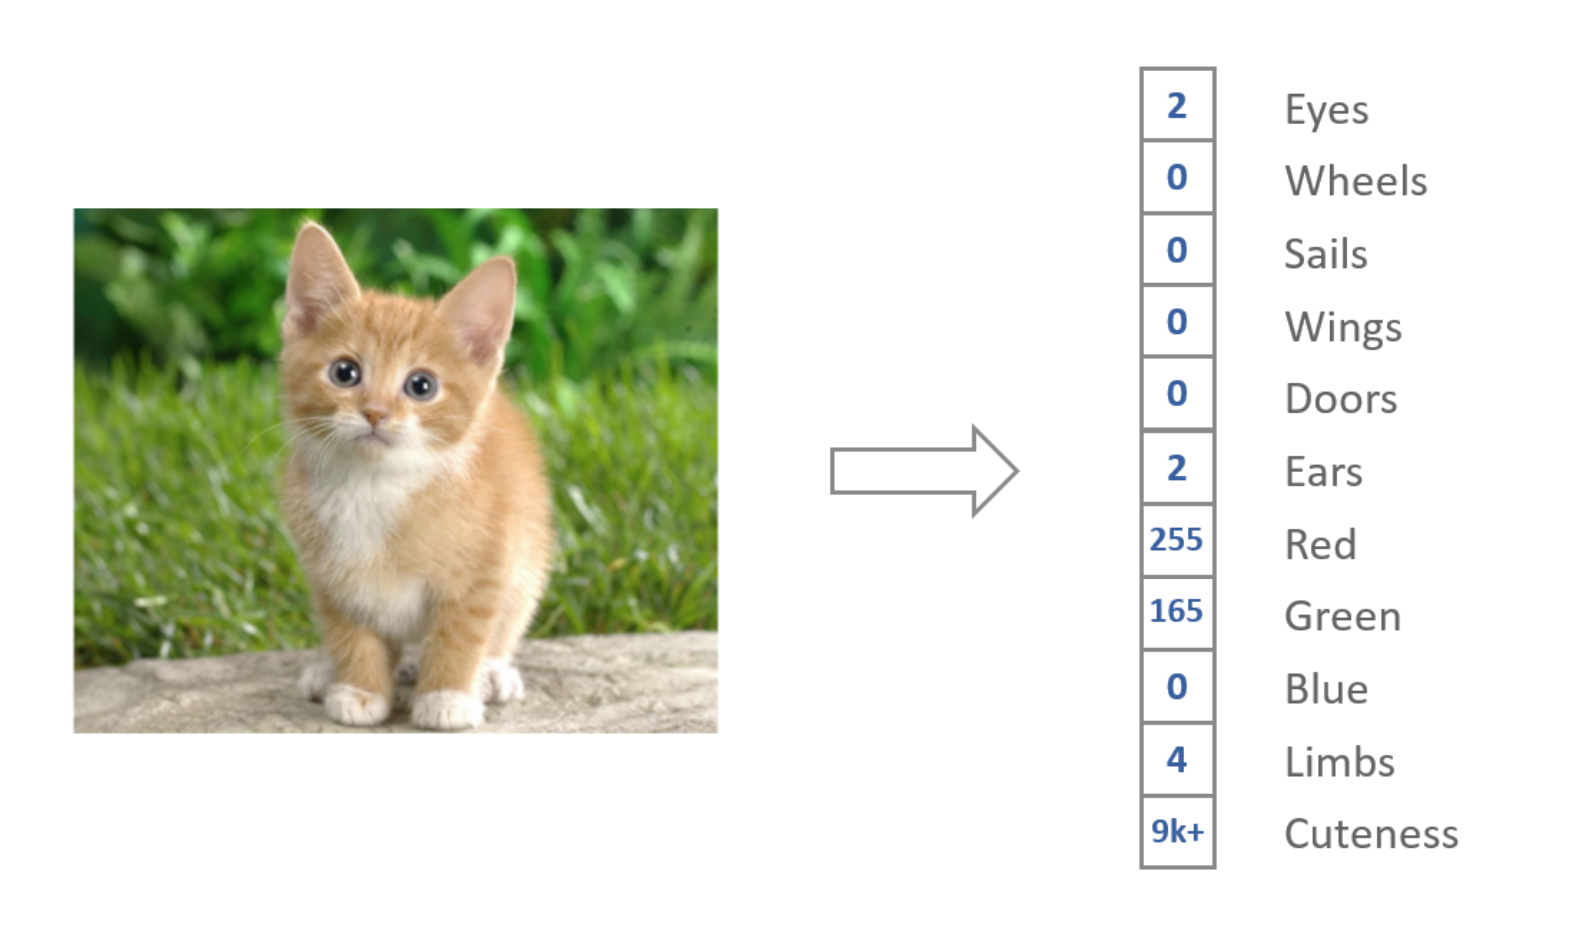
\includegraphics[width=0.5\linewidth]{img/cat_learning.png} 
    \end{figure}
\end{itemize}


\section{Sample Complexity}
The goal of supervised learning is to find the best function $f: \mathcal{X} \rightarrow \mathcal{Y}$ by minimising expected risk

\begin{equation}
    R(f)=\mathbb{E}\left.\ell(f(x),y)=\int_{X\times Y}\ell(f(x),y)\right.d\rho(x,y)
\end{equation}

Given an only finite number of training samples $S=\{(x_1,y_1)\ldots(x_n,y_n)\}$ sampled from $\rho.$
$\rho$ is the unknown data distribution and $\ell$ is the loss function (prediction error). Empirical risk minimisation helps find the best function given our data, by parametrising candidate solutions (for a feature space) as $f(x) = w^\top \phi (x)$, where $w \in \mathcal{H}_\phi$ is a vector of parameters (weights) in a feature space $\mathcal{H}_\phi$. Note that $\phi : \mathcal{X} \rightarrow \mathcal{H}_\phi$ is a feature representation.

\begin{equation}
    \hat{w}=\operatorname*{argmin}_{w\in\mathcal{H}_\phi}\frac1n\sum_{i=1}^n\ell(w^\top\phi(x_i),y_i)
\end{equation}

\begin{definitionbox}{Sample Complexity}
    One way to measure ERM with representation $\phi$ is the \textit{sample complexity}. \\

    It is defined by, for a given $\delta \in [0,1]$ and $\epsilon > 0$, the \textit{sample complexity} of an ERM with representation $\phi$ on a learning problem with data distribution $\rho$ is the minimum number $n_{\delta, \epsilon}(\rho, \phi)$ such that 
    \begin{equation}
        \mathbb{P}\left(R(\hat{w})-\inf_{f:\mathcal{X}\to\mathcal{Y}}R(f)<\varepsilon\right)\geqslant1-\delta 
    \end{equation}
    It is the minimum number of points needed to guarantee ERM performance to be as close as possible to the optimum one within bounds of $\epsilon$, with confidence $1-\delta$.

    The smaller the sample complexity, the better.
\end{definitionbox}

\begin{theorembox}{No Free Lunch Theorem}
\textbf{Basically: }there is no single best universal single feature representation. \\

For any feature representation \( \phi \), there is no guarantee that a small \( n(\rho, \phi) \) exists for all problems, i.e., there is no universal representation that works best for all possible distributions \( \rho \) that we might encounter.\\


The NFLT can be illustrated by considering two different problems, represented by two distributions \( \rho_1 \) and \( \rho_2 \), where the feature representation \( \phi \) leads to a small sample complexity \( n(\rho_1, \phi) \) but may not lead to a similarly small \( n(\rho_2, \phi) \). In essence, what works for one problem may not work for another if the underlying distributions of the data are significantly different.\\

In more formal terms, the NFLT states that the averaged performance of any two algorithms across all possible problems is identical. This implies that an algorithm that performs well on one class of problems must pay for it with degraded performance on the rest of the problems.\\

For any representation $\phi$, we have
\begin{equation}
    \text{sup}_\rho(\rho, \phi)= +\infty
\end{equation}


Overall, the No Free Lunch Theorem emphasises the importance of choosing the right model and representation for the specific problem at hand. It implies that while certain models may perform exceptionally well on certain tasks, their performance may degrade on others, and thus, no single model is superior in all contexts.\\

    \begin{figure}[H]
        \centering
        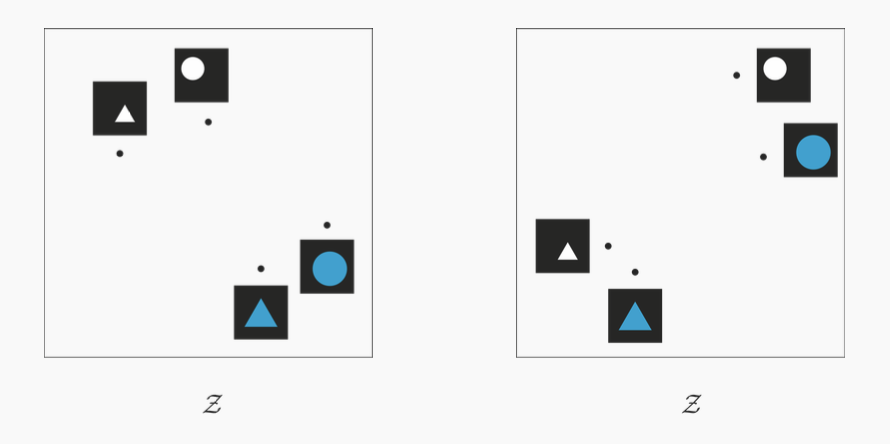
\includegraphics[width=0.65\linewidth]{img/no_free_lunch.png}
        \caption{Either one representation is good for discerning colours, or one representation is good for discerning shapes from others. But there is no universally best representation.}
    \end{figure}
\end{theorembox}

Since there is no best representation $\phi$ for any problem, it is better learn it for the unknown distribution at hand, $rho$ instead of assuming it \textit{a priori}. We can use unlabelled data points. This is the crux of Data Representation Learning, where for each $\phi$ we try to learn $\phi_\rho$.

\section{Representation Learning}
Goal: For feature representation $\phi$ and label predictor $g$, we want to learn $f(x) = g(\phi(x))$. $g$ requires output labels for learning, but $\phi$ does not. By utilising \textbf{reconstruction error}, it is a form of self-supervision.

Denote reconstruction error by 

\begin{equation}
\quad\|x-\psi(\phi(x))\|^2
\end{equation}

Where $\phi$ is now called feature encoding, and $\psi$ is feature decoding.

\begin{figure}[H]
    \centering
    \begin{subfigure}[b]{0.30\textwidth}
        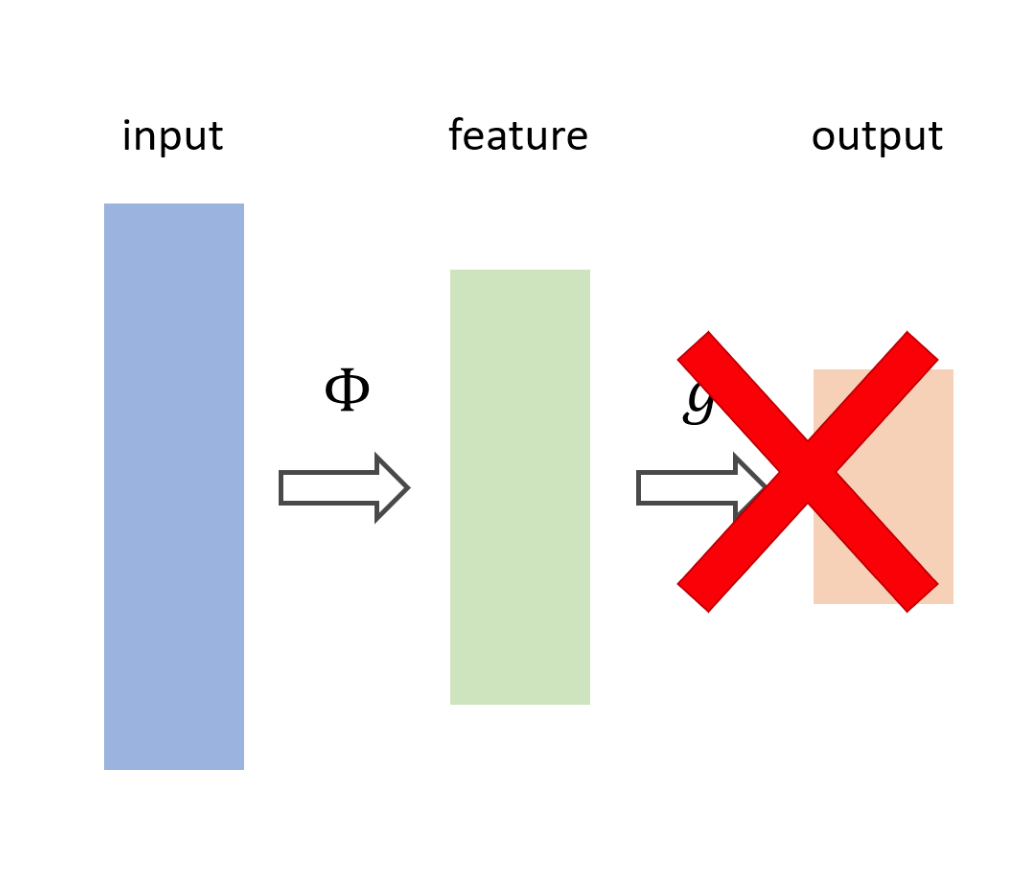
\includegraphics[width=\linewidth]{img/supervised_comparison.png}
        \caption{Typical supervised learning with labelled data}
    \end{subfigure}
    \begin{subfigure}[b]{0.30\textwidth}
        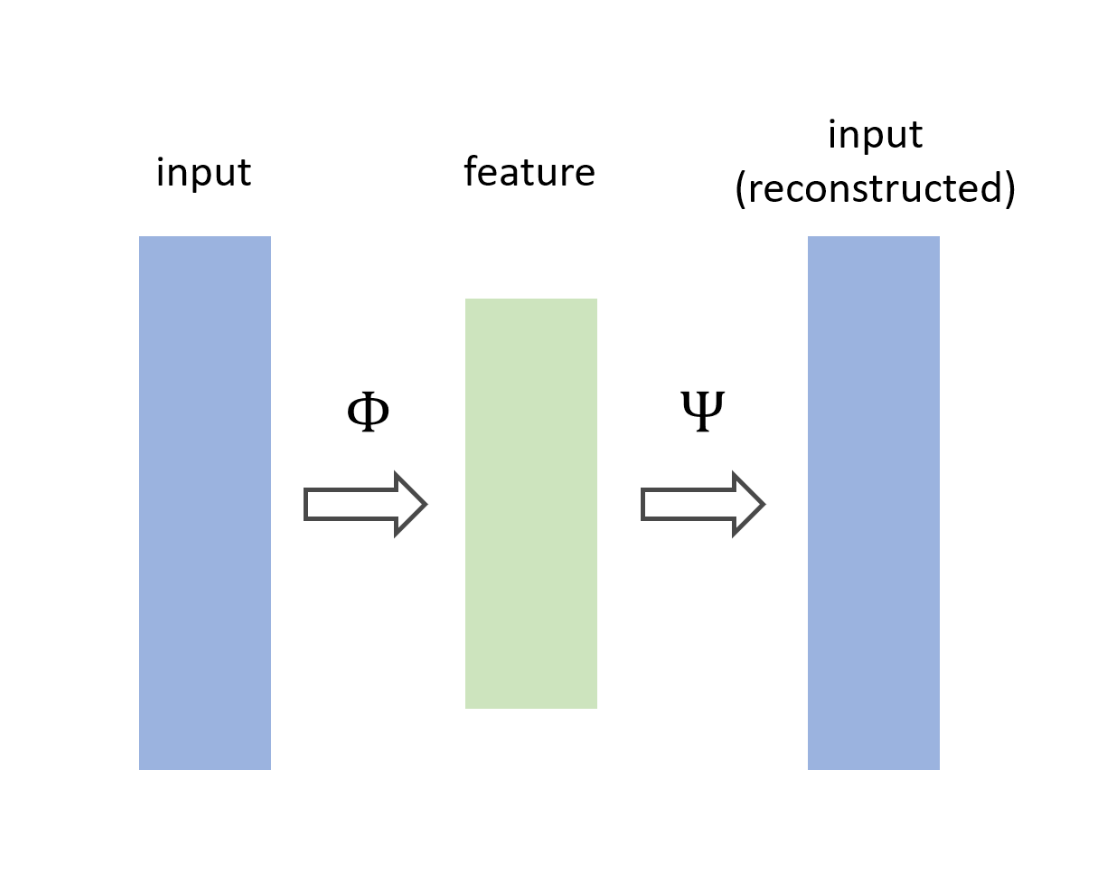
\includegraphics[width=\linewidth]{img/representation_learning.png}
        \caption{Reconstruction of input given unlabelled data}
    \end{subfigure}
\end{figure}

$\phi$ captures more general properties of the data and can be used for other tasks. And learning it is inexpensive due to not requiring labelled data.

\subsection{Training Autoencoders}
Given dataset of $n$ points $(x_i)_{i=1}^n$, we want to solve
\begin{equation}
    \arg\min_{\phi,\psi}\frac1n\sum_{i=1}^n\|x_i-\psi(\phi(x_i))\|^2
\end{equation}

The issue is the trivial solution $\psi \circ \phi$, which is the identity function. For unconstrained $\phi$ and $\psi$ an autoencoder can `learn' all possible variability in training data, which is overfitting it in some sense. More formally, an autoencoder's latent representation captures all variability in the training data, which includes noise. Overfitting occurs when noise is learned instead of the optimum hypothesis that minimises loss.\\

This arises from the capacity of neural networks to approximate any function given enough parameters (as per the Universal Approximation Theorem). If the autoencoder simply learns the identity mapping, it will perfectly reconstruct the inputs without learning any useful or compressed representation of the data.\\

It is ideal to capture only key aspects in the data but ignore noise and nuances, in line with the Efficient Coding Hypothesis from the neuroscience of vision. 

\begin{definitionbox}{Efficient Coding Hypothesis}
    “...the Efficient Coding Hypothesis holds that the purpose of early visual processing is to produce an efficient representation of the incoming visual signal.”(Simoncelli ’03)
    \begin{figure}[H]
        \centering
        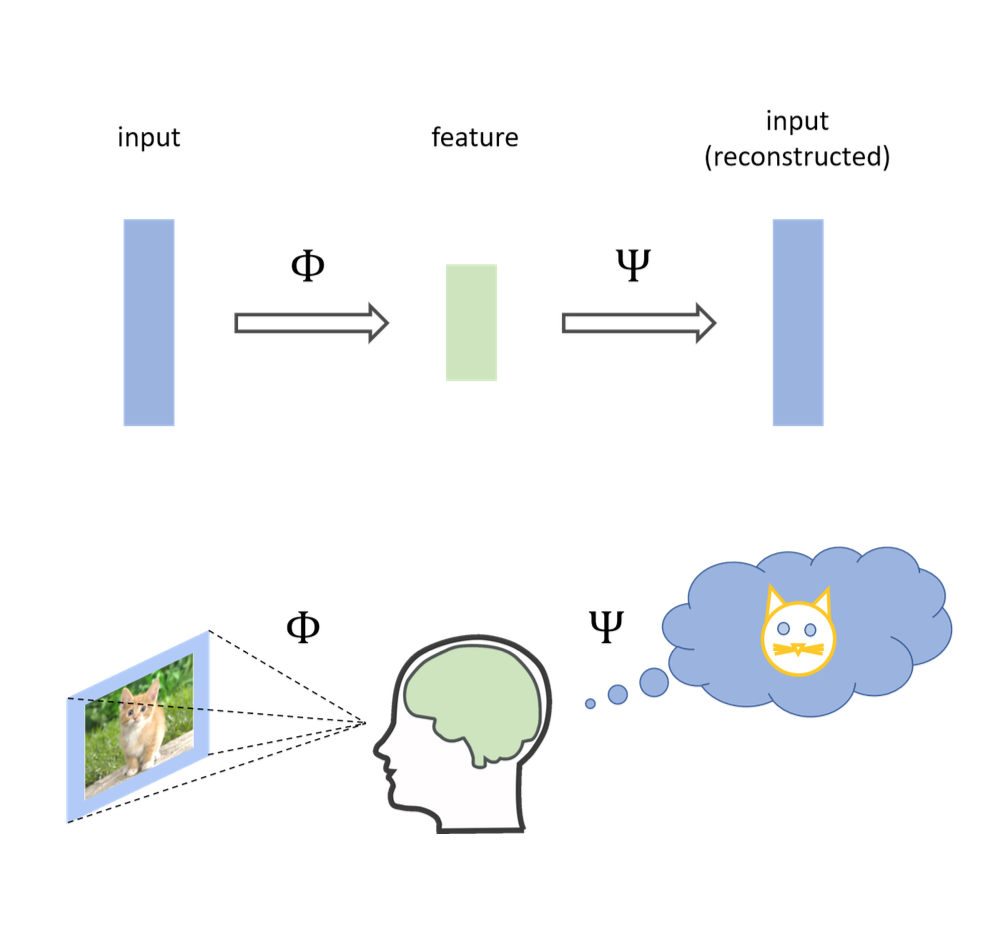
\includegraphics[width=0.5\linewidth]{img/ECH.png}
        
        
    \end{figure}
\end{definitionbox}

\section{Linear Autoencoders}
In general, this course considers Autoencoders wehre $\phi$ and $\psi$ are deep nets. However, the best way is to understand how shallow, linear autoencoders work. They have one hidden layer and no activation function.

Given a dataset of \( n \) points \( \{x_i\}_{i=1}^n \), the objective in training an autoencoder is to solve the following optimisation problem:

\begin{equation}
    \min_{\phi, \psi} \frac{1}{n} \sum_{i=1}^{n} \|x_i - \psi(\phi(x_i))\|^2
\end{equation}

where \( \phi : \mathbb{R}^d \to \mathbb{R}^r \) and \( \psi : \mathbb{R}^r \to \mathbb{R}^d \) correspond to matrices \( F, P \in \mathbb{R}^{r \times d} \), such that:

\begin{equation}
    \psi(\phi(x)) = P^TFx
\end{equation}



Note that the matrix \( P^TF \) is \( d \times d \) of rank at most \( r \leq d \). If \( r < d \), then \( P^TF \) cannot be the identity matrix.

The problem of training a linear Autoencoder becomes,

\begin{equation}
    \min_{P, F \in \mathbb{R}^{d \times r}} \frac{1}{n} \sum_{i=1}^{n} \|x_i - P^T Fx_i\|^2 = \min_{P, F \in \mathbb{R}^{d \times r}} \frac{1}{n} \|\mathbf{X} - P^T F\mathbf{X}\|_F^2
\end{equation}

Here, \( \mathbf{X} = [x_1, \ldots, x_n] \in \mathbb{R}^{d \times n} \) is the matrix concatenating the input data, and \( \|\mathbf{M}\|_F^2 = \text{Tr}(\mathbf{MM}^T) \) is the squared Frobenius norm of a matrix \( \mathbf{M} \) (sum of squared entries).


\begin{theorembox}{Principal Component Analysis}
    The solution $\hat{P} ^T \hat{F}$ encodes the first $r$ principal components of the data.\\

    $P ^\top F$ is learning an orthogonal projector onto a linear subspace of dimension $r$. 
    \begin{enumerate}
    \item Set the derivative of the objective function with respect to \( F \) to zero:
    \[ 0 = \nabla_F \|X - P^T FX\|_F^2 = 2P(X - P^T FX)X^T = 2(P - PP^T F)XX^T \]
    
    \item Solving \( P - PP^T F = 0 \) gives us \( F = (P^T P)^{+}P = (P^T)^+\), the psuedoinverse of $P^T$.
    
    \item Hence, we have \( P^T F = P^T (P^T )^{+} = \Pi \) which is an orthogonal projector onto the range of \( P \).
\end{enumerate}

Given that \( \Pi = P^T F \) is an orthogonal projector, we have \( \Pi^2 = \Pi \), and it can be associated with the first \( r \) principal components of \( X \).

\begin{enumerate}
    \item For a projector \( \Pi \), we have \( \Pi^2 = \Pi \). Hence, \( (I - \Pi)(I - \Pi) = I - \Pi \).
    
    \item Therefore, the reconstruction error simplifies to:
    \[ \|X - P^T FX\|_F^2 = \|(I - \Pi)X\|_F^2 = \text{Tr}(X^T (I - \Pi)X) \]
    
    \item Recall that an orthogonal projector of rank \( r \) can be written as \( \Pi = UU^T \), where \( U \) is a matrix with orthonormal columns.
    
    \item Hence, the trace simplifies further:
    \[ \text{Tr}(X^T (I - \Pi)X) = \text{Tr}(X^T X) - \text{Tr}(X^T UU^T X) \]
\end{enumerate}

The training of an autoencoder can be recast as a matrix factorisation problem:

\begin{equation}
\min_{F,P} \|X - P^T F\|_F^2 = \min_{U \in \mathbb{R}^{d \times r}, U^T U = I} \text{Tr}(X^T X) - \text{Tr}(U^T X^T X U) = \max_{U \in \mathbb{R}^{d \times r}, U^T U = I} \text{Tr}(U^T X^T X U)
\end{equation}

Here, the trace of \( U^T X^T X U \) is given by:

\begin{equation}
\text{Tr}(U^T X^T X U) = \sum_{j=1}^{r} u_j^T X^T X u_j,
\end{equation}


with \( u_j \) being the \( j \)-th column of \( U \).

Recall that \( \max_{||u||=1}u^T X^T X u \)  is attained by the first principal component of \( X \). Thus, the optimisation problem becomes:

\begin{equation}
\min_{F,P} \|X - P^T F\|_F^2 = \max_{U^T U = I} \sum_{j=1}^{r} u_j^T X^T X u_j,
\end{equation}

which is equivalent to finding the first \( r \) principal components of \( X \).


    
\end{theorembox}

\subsection{Nonlinear Features}
When working with linear encoders, we can consider a feature transformation $\phi$ to capture non-linear relations in the data, if we know such nonlinear relations beforehand. 

\begin{figure}[H]
    \centering
    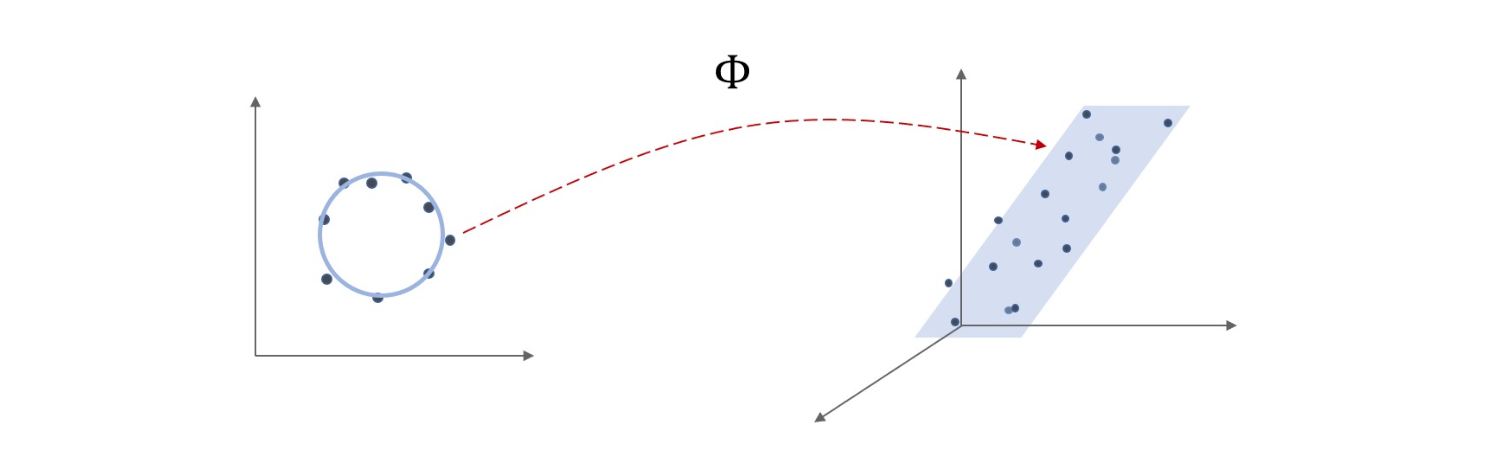
\includegraphics[width=0.5\linewidth]{img/PCA_transform.png}
\end{figure}

If $\phi$ is not known, a deep, nonlinear autoencoder can be used to learn it.

\begin{figure}[H]
    \centering
    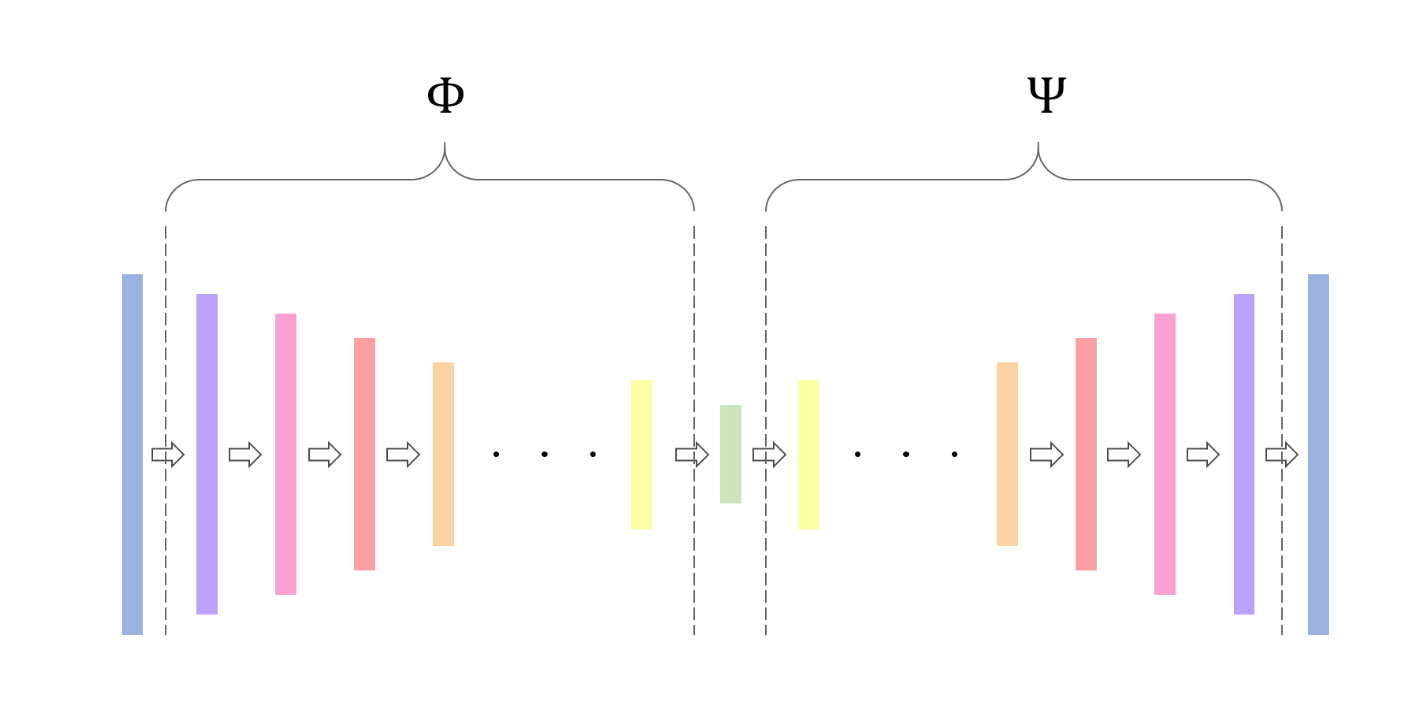
\includegraphics[width=0.5\linewidth]{img/d_nonlinear_autoencoder.png}
    
    
\end{figure}